\bta{测定金属的电阻率}


\begin{enumerate}
%\renewcommand{\labelenumi}{\arabic{enumi}.}
% A(\Alph) a(\alph) I(\Roman) i(\roman) 1(\arabic)
%设定全局标号series=example	%引用全局变量resume=example
%[topsep=-0.3em,parsep=-0.3em,itemsep=-0.3em,partopsep=-0.3em]
%可使用leftmargin调整列表环境左边的空白长度 [leftmargin=0em]
\item
\exwhere{$ 2012 $年理综山东卷}
在测量金属丝电阻率的实验中,可供选用的器材如下:\\
待测金属丝:$ R_{x} $(阻值约$ 4 \ \Omega $,额定电流约$ 0.5 \ A $);\\
电压表:$ V $(量程$ 3 \ V $,内阻约$ 3 \ k\Omega $);\\
电流表:$ A_{1} $(量程$ 0.6 \ A $,内阻约$ 0.2 \ \Omega $); \quad $ A_{2} $(量程$ 3 \ A $,内阻约$ 0.05 \ \Omega $);\\
电源:$ E_{1} $(电动势$ 3 \ V $,内阻不计); \quad $ E_{2} $(电动势$ 12 \ V $,内阻不计)\\
滑动变阻器:$ R $(最大阻值约$ 20 \ \Omega $)\\
螺旋测微器;毫米刻度尺;开关$ S $;导线。



\begin{enumerate}
%\renewcommand{\labelenumi}{\arabic{enumi}.}
% A(\Alph) a(\alph) I(\Roman) i(\roman) 1(\arabic)
%设定全局标号series=example	%引用全局变量resume=example
%[topsep=-0.3em,parsep=-0.3em,itemsep=-0.3em,partopsep=-0.3em]
%可使用leftmargin调整列表环境左边的空白长度 [leftmargin=0em]
\item
用螺旋测微器测量金属丝的直径,示数如图所示,读数为
\underlinegap 
$ mm $。
\begin{figure}[h!]
\centering
\includesvg[width=0.23\linewidth]{picture/svg/GZ-3-tiyou-0959}
\end{figure}

\item 
若滑动变阻器采用限流接法,为使测量尽量精确,电流表应选
\underlinegap 
、电源应选
\underlinegap 
(均填器材代
号),在虚线框中完成电路原理图。
\begin{figure}[h!]
\centering
\includesvg[width=0.23\linewidth]{picture/svg/GZ-3-tiyou-0960}
\end{figure}


\end{enumerate}

\tk{
\begin{enumerate}
%\renewcommand{\labelenumi}{\arabic{enumi}.}
% A(\Alph) a(\alph) I(\Roman) i(\roman) 1(\arabic)
%设定全局标号series=example	%引用全局变量resume=example
%[topsep=-0.3em,parsep=-0.3em,itemsep=-0.3em,partopsep=-0.3em]
%可使用leftmargin调整列表环境左边的空白长度 [leftmargin=0em]
\item
$ 1.773 $ ($ 1.771 \sim 1.775 $均正确)
\item 
$ A_{1} $ \quad $ E_{1} $\\
电路如图所示
\begin{center}
\includesvg[width=0.23\linewidth]{picture/svg/GZ-3-tiyou-0968} 	
\end{center}
\end{enumerate}
} 


\item 
\exwhere{$ 2012 $ 年理综广东卷}
某同学测量一个圆柱体的电阻率,需要测量圆柱体的尺寸和电阻。
\begin{figure}[h!]
\centering
\begin{subfigure}{0.4\linewidth}
\centering
\includesvg[width=0.7\linewidth]{picture/svg/GZ-3-tiyou-0961} 
\caption{}\label{}
\end{subfigure}
\begin{subfigure}{0.4\linewidth}
\centering
%\includesvg[width=0.7\linewidth]{picture/svg/GZ-3-tiyou-0962}
 \includesvg[width=0.7\linewidth]{picture/svg/GZ-3-tiyou-0963} 
\caption{}\label{}
\end{subfigure}
\begin{subfigure}{0.4\linewidth}
\centering
\includesvg[width=0.7\linewidth]{picture/svg/GZ-3-tiyou-0964} 
\caption{}\label{}
\end{subfigure}
\end{figure}

\begin{enumerate}
%\renewcommand{\labelenumi}{\arabic{enumi}.}
% A(\Alph) a(\alph) I(\Roman) i(\roman) 1(\arabic)
%设定全局标号series=example	%引用全局变量resume=example
%[topsep=-0.3em,parsep=-0.3em,itemsep=-0.3em,partopsep=-0.3em]
%可使用leftmargin调整列表环境左边的空白长度 [leftmargin=0em]
\item
分别使用游标卡尺和螺旋测微器测量圆柱体的长度和直径,某次测量的示数如图($ a $)和图 ($ b $)所示,长度为 \underlinegap $ cm $,直径为 \underlinegap $ mm $。



\item 
按图($ c $)连接电路后,实验操作如下:
\begin{enumerate}
%\renewcommand{\labelenumi}{\arabic{enumi}.}
% A(\Alph) a(\alph) I(\Roman) i(\roman) 1(\arabic)
%设定全局标号series=example	%引用全局变量resume=example
%[topsep=-0.3em,parsep=-0.3em,itemsep=-0.3em,partopsep=-0.3em]
%可使用leftmargin调整列表环境左边的空白长度 [leftmargin=0em]
\item
将滑动变阻器 $ R_{1} $ 的阻值置于最 \underlinegap 处(填“大”或“小”);将 $ S_{2} $ 拨向接点 $ 1 $,闭合 $ S_{1} $,调节
$ R_{1} $,使电流表示数为 $ I_{0} $;


\item 
将电阻箱$ R_{2} $的阻值调至最 \underlinegap (填“大”或“小”);将$ S_{2} $拨向接点$ 2 $;保持$ R_{1} $不变,调节$ R_{2} $,使
电流表示数仍为$ I_{0} $,此时$ R_{2} $阻值为$ 1280 \ \Omega $;

\end{enumerate}




\item 
由此可知,圆柱体的电阻为 \underlinegap $ \Omega $。


\end{enumerate}

\tk{
\begin{enumerate}
%\renewcommand{\labelenumi}{\arabic{enumi}.}
% A(\Alph) a(\alph) I(\Roman) i(\roman) 1(\arabic)
%设定全局标号series=example	%引用全局变量resume=example
%[topsep=-0.3em,parsep=-0.3em,itemsep=-0.3em,partopsep=-0.3em]
%可使用leftmargin调整列表环境左边的空白长度 [leftmargin=0em]
\item
$ 5.01 $ \quad $ 5.315 $
\item 
大 \quad 大 
\item 
$ 1280 $
\end{enumerate}
} 



\item 
\exwhere{$ 2013 $ 年安徽卷}
\begin{enumerate}
%\renewcommand{\labelenumi}{\arabic{enumi}.}
% A(\Alph) a(\alph) I(\Roman) i(\roman) 1(\arabic)
%设定全局标号series=example	%引用全局变量resume=example
%[topsep=-0.3em,parsep=-0.3em,itemsep=-0.3em,partopsep=-0.3em]
%可使用leftmargin调整列表环境左边的空白长度 [leftmargin=0em]
\item
在测定一根粗细均匀合金丝电阻
率的实验中,利用螺旋测微器测定合金丝直径的过程
如图所示,校零时的读数为 \underlinegap $ mm $,合金丝的
直径为 \underlinegap $ mm $。
\begin{figure}[h!]
\centering
\includesvg[width=0.23\linewidth]{picture/svg/GZ-3-tiyou-0965}
\end{figure}

\item 
为了精确测量合金丝的电阻 $ R_{x} $,设计出如图 $ 1 $ 所
示的实验电路图,按照该电路图完成图 $ 2 $ 中的实物电路连接。
\begin{figure}[h!]
\centering
\begin{subfigure}{0.4\linewidth}
\centering
\includesvg[width=0.7\linewidth]{picture/svg/GZ-3-tiyou-0966} 
\caption{}\label{}
\end{subfigure}
\begin{subfigure}{0.4\linewidth}
\centering
%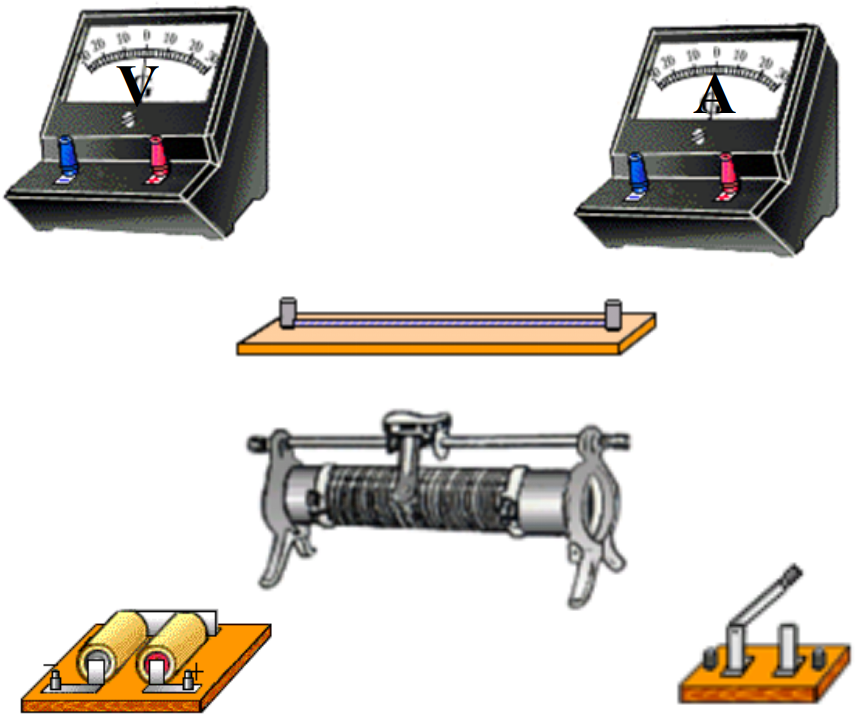
\includegraphics[width=0.7\linewidth]{picture/screenshot057}
\includesvg[width=0.7\linewidth]{picture/svg/GZ-3-tiyou-0967} 
\caption{}\label{}
\end{subfigure}
\end{figure}




\end{enumerate}

\tk{
\begin{enumerate}
%\renewcommand{\labelenumi}{\arabic{enumi}.}
% A(\Alph) a(\alph) I(\Roman) i(\roman) 1(\arabic)
%设定全局标号series=example	%引用全局变量resume=example
%[topsep=-0.3em,parsep=-0.3em,itemsep=-0.3em,partopsep=-0.3em]
%可使用leftmargin调整列表环境左边的空白长度 [leftmargin=0em]
\item
$ 0.007 \quad 0.638 $
\item 
如图所示
\begin{center}
%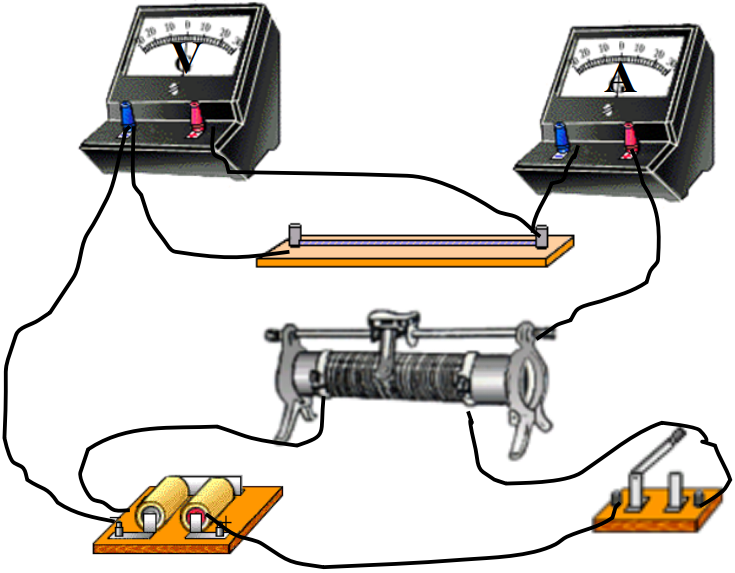
\includegraphics[width=0.7\linewidth]{picture/screenshot058}
\includesvg[width=0.23\linewidth]{picture/svg/GZ-3-tiyou-0969} 
\end{center}	
\end{enumerate}
} 



\item 
\exwhere{$ 2012 $ 年理综北京卷}
在“测定金属的电阻率”实验中,所用测量仪器均已校准,待测金属丝接入电路部分的长度约为
$ 50 \ cm $。
\begin{figure}[h!]
\centering
\begin{subfigure}{0.4\linewidth}
\centering
%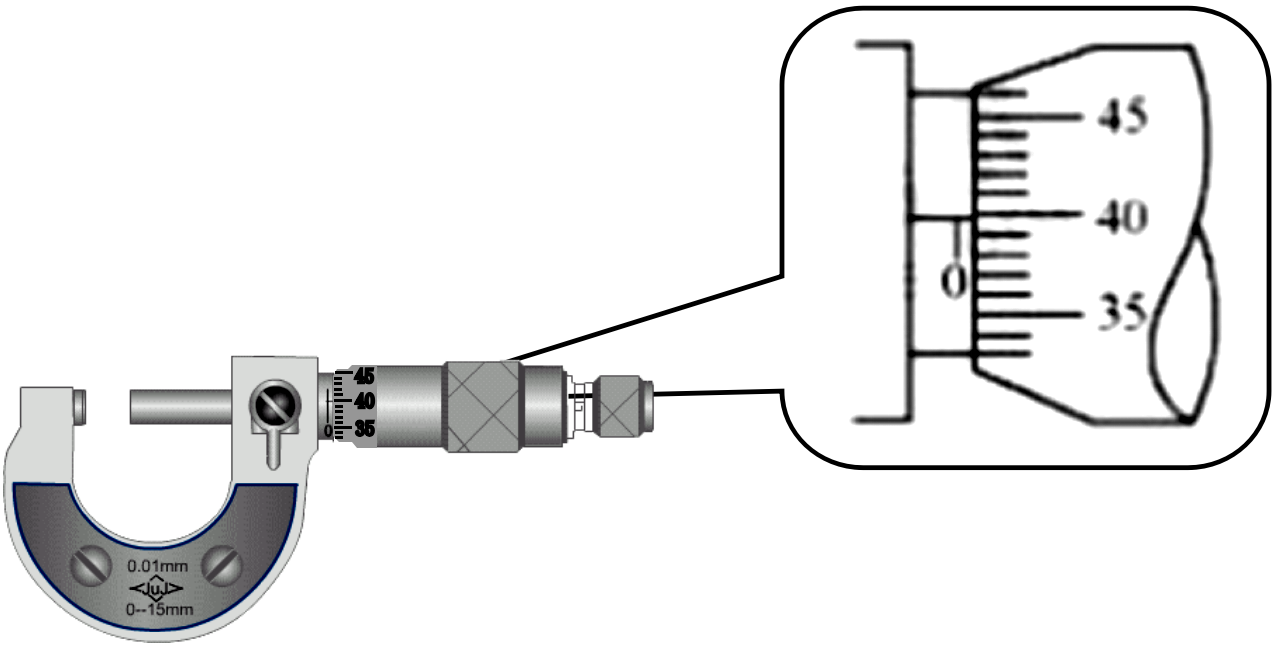
\includegraphics[width=0.7\linewidth]{picture/screenshot059}
\includesvg[width=0.7\linewidth]{picture/svg/GZ-3-tiyou-0970} 
\caption{}\label{}
\end{subfigure}
\begin{subfigure}{0.4\linewidth}
\centering
\includesvg[width=0.7\linewidth]{picture/svg/GZ-3-tiyou-0971} 
\caption{}\label{}
\end{subfigure}
\begin{subfigure}{0.4\linewidth}
\centering
\includesvg[width=0.7\linewidth]{picture/svg/GZ-3-tiyou-0972} 
\caption{}\label{}
\end{subfigure}
\begin{subfigure}{0.4\linewidth}
\centering
\includesvg[width=0.7\linewidth]{picture/svg/GZ-3-tiyou-0973} 
\caption{}\label{}
\end{subfigure}
\end{figure}

\begin{enumerate}
%\renewcommand{\labelenumi}{\arabic{enumi}.}
% A(\Alph) a(\alph) I(\Roman) i(\roman) 1(\arabic)
%设定全局标号series=example	%引用全局变量resume=example
%[topsep=-0.3em,parsep=-0.3em,itemsep=-0.3em,partopsep=-0.3em]
%可使用leftmargin调整列表环境左边的空白长度 [leftmargin=0em]
\item
用螺旋测微器测量金属丝的直径,其中某一次测量结果如图 $ 1 $ 所示,其读数应为
\underlinegap 
$ mm $
(该值接近多次测量的平均值)
。

\item 
用伏安法测金属丝的电阻 $ R_{x} $。实验所用器材为:电池组(电动势 $ 3 \ V $,内阻约 $ 1 \ \Omega $)、电流表
(内阻约 $ 0.1 \ \Omega $)、电压表(内阻约 $ 3 \ k\Omega $)、滑动变阻器 $ R $($ 0 \sim 20 \ \Omega $,额定电流 $ 2 \ A $)、开关、导线若
干。

某小组同学利用以上器材正确连接好电路,进行实验测量,记录数据如下:
\begin{table}[h!]
\centering 
\begin{tabular}{|c|c|c|c|c|c|c|c|}
\hline 
次数 & $ 1 $ & $ 2 $ & $ 3 $ & $ 4 $ & $ 5 $ & $ 6 $ & $ 7 $
 \\
\hline
$ U/V $ & $ 0.10 $ & $ 0.30 $ & $ 0.70 $ & $ 1.00 $ & $ 1.50 $ & $ 1.70 $ & $ 2.30 $
 \\
\hline
$ I/A $ & $ 0.020 $ & $ 0.060 $ & $ 0.160 $ & $ 0.220 $ & $ 0.340 $ & $ 0.460 $ & $ 0.520 $\\ 
\hline 
\end{tabular}
\end{table} 


由以上实验数据可知,他们
测量 $ R_{x} $ 是采用图 $ 2 $ 中的 \underlinegap 
图(选填“甲”或“乙”)
。

\item 
图 $ 3 $ 是测量 $ R_{x} $ 的实验器材实物图,图中已连接了部分导线,滑动变阻器的滑片 $ P $ 置于变阻器
的一端。请根据($ 2 $)所选的电路图,补充完成图 $ 3 $ 中实物间的连线,并使闭合开关的瞬间,电压
表或电流表不至于被烧坏。


\item 
这个小组的同学在坐标纸上建立 $ U $、$ I $ 坐标系,如图 $ 4 $ 所示,图中已标出了与测量数据对应的
$ 4 $个坐标点。请在图 $ 4 $ 中标出第 $ 2 $、$ 4 $、$ 6 $ 次测量数据的坐标点,并描绘出 $ U-I $ 图线。由图线得到金
属丝的阻值 $ R_{x} = $ \underlinegap 
$ \Omega $(保留两位有效数字)。

\item 
根据以上数据可以估算出金属丝电阻率约为
\underlinegap 
(填选项前的符号)。

\fourchoices
{$ 1 \times 10^{-2} \ \Omega \cdot m $}
{$ 1 \times 10^{-3} \ \Omega \cdot m $}
{$ 1 \times 10^{-6} \ \Omega \cdot m $}
{$ 1 \times 10^{-8} \ \Omega \cdot m $}

\item 
任何实验测量都存在误差。本实验所用测量仪器均已校准,下列关于误差的说法中正确的选
项是
\underlinegap 
(有多个正确选项)。

\fourchoices
{用螺旋测微器测量金属丝直径时,由于读数引起的误差属于系统误差}
{由于电流表和电压表内阻引起的误差属于偶然误差}
{若将电流表和电压表的内阻计算在内,可以消除由测量仪器引起的系统误差}
{用 $ U-I $ 图像处理数据求金属丝电阻可以减小偶然误差}



\end{enumerate}


\tk{
\begin{enumerate}
%\renewcommand{\labelenumi}{\arabic{enumi}.}
% A(\Alph) a(\alph) I(\Roman) i(\roman) 1(\arabic)
%设定全局标号series=example	%引用全局变量resume=example
%[topsep=-0.3em,parsep=-0.3em,itemsep=-0.3em,partopsep=-0.3em]
%可使用leftmargin调整列表环境左边的空白长度 [leftmargin=0em]
\item
$ 0.397 \ mm $ \quad $ (0.395 \sim 0.399) $
\item 
甲
\item 
如图所示
\begin{center}
 \includesvg[width=0.23\linewidth]{picture/svg/GZ-3-tiyou-0974} 
\end{center}
\item 
$ R_{x}=4.5 \ \Omega $ \quad ($ 4.3 \sim 4.7 $),电路如图
\begin{center}
 \includesvg[width=0.23\linewidth]{picture/svg/GZ-3-tiyou-0975} 
\end{center}
\item 
C
\item 
CD
\end{enumerate}
} 


\item
\exwhere{$ 2014 $ 年物理江苏卷}
某同学通过实验测量一种合金的电阻率。
\begin{figure}[h!]
\centering
\begin{subfigure}{0.4\linewidth}
\centering
\includesvg[width=0.7\linewidth]{picture/svg/GZ-3-tiyou-0976} 
\caption{}\label{}
\end{subfigure}
\begin{subfigure}{0.55\linewidth}
\centering
%\includesvg[width=0.99\linewidth]{picture/svg/GZ-3-tiyou-0977} 
 \includesvg[width=0.99\linewidth]{picture/svg/GZ-3-tiyou-0978} 
\caption{}\label{}
\end{subfigure}
\end{figure}

\begin{enumerate}
%\renewcommand{\labelenumi}{\arabic{enumi}.}
% A(\Alph) a(\alph) I(\Roman) i(\roman) 1(\arabic)
%设定全局标号series=example	%引用全局变量resume=example
%[topsep=-0.3em,parsep=-0.3em,itemsep=-0.3em,partopsep=-0.3em]
%可使用leftmargin调整列表环境左边的空白长度 [leftmargin=0em]
\item
用螺旋测微器测量合金丝的直径。 为防止读数时测微螺杆发生转动,读数前应先旋紧
图$ a $所示的部件 \underlinegap 
(选填“ “$ A $”、“ “$ B $” 、“ “$ C $” 或“ “$ D $” ) 。 从图中的示数可读出合金丝的直径为 \underlinegap 
$ mm $。


\item 
图$ 2 $所示是测量合金丝电阻的电路,相关器材的规格已在图中标出。合上开关,将滑动
变阻器的滑片移到最左端的过程中,发现电压表和电流表的指针只在图示位置发生很小的变化。
由此可以推断:电路中 \underlinegap 
( 选填图中表示接线柱的数字) 之间出现了 \underlinegap 
( 选填“ “短路” 或 “断路” )。

\item 
在电路故障被排除后,调节滑动变阻器,读出电压表和电流表的示数分别为 $ 2.23 \ V $ 和 $ 38 \ mA $,
由此,该同学算出接入电路部分的合金丝的阻值为 $ 58.7 \ \Omega $. 为了更准确地测出合金丝的阻值,在
不更换实验器材的条件下,对实验应作怎样的改进? 请写出两条建议:

\hfullline 



\end{enumerate}


\tk{
\begin{enumerate}
%\renewcommand{\labelenumi}{\arabic{enumi}.}
% A(\Alph) a(\alph) I(\Roman) i(\roman) 1(\arabic)
%设定全局标号series=example	%引用全局变量resume=example
%[topsep=-0.3em,parsep=-0.3em,itemsep=-0.3em,partopsep=-0.3em]
%可使用leftmargin调整列表环境左边的空白长度 [leftmargin=0em]
\item
$ B \quad 0.410 $
\item 
$ 7 $、$ 9 $ \quad 断路
\item 
电流表改为内接;测量多组电流和电压值,计算出电阻的平均值(或多测几组电流值和电压
值,用图象法求电阻值)
\end{enumerate}
} 

\item 
\exwhere{$ 2019 $ 年物理江苏卷}
某同学测量一段长度已知的电阻丝的电阻率.实验操作如下:
\begin{enumerate}
%\renewcommand{\labelenumi}{\arabic{enumi}.}
% A(\Alph) a(\alph) I(\Roman) i(\roman) 1(\arabic)
%设定全局标号series=example	%引用全局变量resume=example
%[topsep=-0.3em,parsep=-0.3em,itemsep=-0.3em,partopsep=-0.3em]
%可使用leftmargin调整列表环境左边的空白长度 [leftmargin=0em]
\item
螺旋测微器如题 $ 1 $ 图所示.在测量电阻丝直径时,先将电阻丝轻轻地夹在测砧与测微螺杆之
间,再旋动 \underlinegap (选填“$ A $”“$ B $”或“$ C $”),直到听见“喀喀”的声音,以保证压力适当,同时防止螺旋
测微器的损坏。
\begin{figure}[h!]
\centering
\includesvg[width=0.53\linewidth]{picture/svg/GZ-3-tiyou-0979}
\end{figure}

\item 
选择电阻丝的 \underlinegap (选填“同一”或“不同”)位置进行多次测量,取其平均值作为电阻丝的直
径。

\item 
$ 2 $ 图甲中 $ R_{x} $,为待测电阻丝.请用笔画线代替导线,将滑动变阻器接入 $ 2 $ 图乙实物电路中的
正确位置 \underlinegap 。
\begin{figure}[h!]
\centering
\begin{subfigure}{0.4\linewidth}
\centering
\includesvg[width=0.7\linewidth]{picture/svg/GZ-3-tiyou-0981} 
\caption{}\label{}
\end{subfigure}
\begin{subfigure}{0.4\linewidth}
\centering
\includesvg[width=0.7\linewidth]{picture/svg/GZ-3-tiyou-0982} 
\caption{}\label{}
\end{subfigure}
\end{figure}



\item 
为测量 $ R $,利用 $ 2 $ 图甲所示的电路,调节滑动变阻器测得 $ 5 $ 组电压 $ U_{1} $ 和电流 $ I_{1} $ 的值,作出的
$ U_{1} - I_{1} $ 关系图象如图图所示.接着,将电压表改接在 $ a $、$ b $ 两端,测得 $ 5 $ 组电压 $ U_{2} $ 和电流 $ I_{2} $ 的值,数据见下表:
\begin{table}[h!]
\centering 
\begin{tabular}{|l|l|l|l|l|l|}
\hline$U_{2} / V$ & 0.50 & 1.02 & 1.54 & 2.05 & 2.55 \\
\hline$I_{2} / mA$ & 20.0 & 40.0 & 60.0 & 80.0 & 100.0 \\
\hline
\end{tabular}
\end{table} 



请根据表中的数据,在方格纸上作出 $ U_{2} - I_{2} $ 图象。
\begin{figure}[h!]
\centering
\includesvg[width=0.23\linewidth]{picture/svg/GZ-3-tiyou-0980}
\end{figure}

\item 
由此,可求得电阻丝的 $ R_{x} =$ \underlinegap $ \Omega $。根据电阻定律可得到电阻丝的电阻率。



\end{enumerate}


\tk{
\begin{enumerate}
%\renewcommand{\labelenumi}{\arabic{enumi}.}
% A(\Alph) a(\alph) I(\Roman) i(\roman) 1(\arabic)
%设定全局标号series=example	%引用全局变量resume=example
%[topsep=-0.3em,parsep=-0.3em,itemsep=-0.3em,partopsep=-0.3em]
%可使用leftmargin调整列表环境左边的空白长度 [leftmargin=0em]
\item
C
\item 
不同
\item 
如图所示
\begin{center}
\includesvg[width=0.23\linewidth]{picture/svg/GZ-3-tiyou-0983} 
\end{center}
\item 
如图所示
\begin{center}
\includesvg[width=0.23\linewidth]{picture/svg/GZ-3-tiyou-0984} 
\end{center}
\item 
$ 23.5 $($ 23.0 \sim 24.0 $ 都算对)	
\end{enumerate}
} 


\item 
\exwhere{$ 2019 $ 年物理天津卷}
现测定长金属丝的电阻率。
\begin{enumerate}
%\renewcommand{\labelenumi}{\arabic{enumi}.}
% A(\Alph) a(\alph) I(\Roman) i(\roman) 1(\arabic)
%设定全局标号series=example	%引用全局变量resume=example
%[topsep=-0.3em,parsep=-0.3em,itemsep=-0.3em,partopsep=-0.3em]
%可使用leftmargin调整列表环境左边的空白长度 [leftmargin=0em]
\item
某次用螺旋测微器测量金属丝直径 的结果如图所示,其读数是 \underlinegap $ mm $。
\begin{figure}[h!]
\centering
\includesvg[width=0.23\linewidth]{picture/svg/GZ-3-tiyou-0986}
\end{figure}

\item 
利用下列器材设计一个电路,尽量准确地测量一段金属丝的电阻。这段金属丝的电阻 $ R_{x} $,约为$ 100 \ \Omega $,画出实验电路图,并标明器材代号。

电源 $ E $ \quad (电动势 $ 10 \ V $,内阻约为 $ 10 \ \Omega $ )\\
电流表 $ A_{1} $ \quad (量程 $ 0 \sim 250 \ mA $,内阻 $ R_{1} =5 \ \Omega $ )\\
电流表 $ A_{2} $ \quad (量程 $ 0 \sim 300 \ mA $,内阻约为 $ 5 \ \Omega $ )\\
滑动变阻器 $ R $ \quad (最大阻值 $ 10 \ \Omega $,额定电流 $ 2 \ A $ )\\
开关 $ S $ 及导线若干

\item 
某同学设计方案正确,测量得到电流表 $ A_{1} $ 的读数为 $ I_{1} $,电流表 $ A_{2} $ 的读数为 $ I_{2} $,则这段金属丝
电阻的计算式 $ R_{x} = $ \underlinegap 。从设计原理看,其测量值与真实值相比 \underlinegap (填“偏大”、“偏小”或
“相等”)。




\end{enumerate}

\tk{
\begin{enumerate}
%\renewcommand{\labelenumi}{\arabic{enumi}.}
% A(\Alph) a(\alph) I(\Roman) i(\roman) 1(\arabic)
%设定全局标号series=example	%引用全局变量resume=example
%[topsep=-0.3em,parsep=-0.3em,itemsep=-0.3em,partopsep=-0.3em]
%可使用leftmargin调整列表环境左边的空白长度 [leftmargin=0em]
\item
$ 0.200 $ \quad $(0.196 \sim 0.204$ 均可 $)$
\item 
\begin{center}
\includesvg[width=0.23\linewidth]{picture/svg/GZ-3-tiyou-0987} 
\end{center}
\item 
$\frac{I_{1} R_{1}}{I_{2}-I_{1}}$ \quad 相等
\end{enumerate}
} 





\end{enumerate}

